%%
%% 部:スタンダードレイアウト
%%------------------------------------------------------------------------------------------------------------------------------%%
\part{スタンダードレイアウト}
%%
%% 章:この PART で制作するサイト
%%------------------------------------------------------------------------------------------------------------------------------%%
\chapter{この Part で制作するサイト}
この Part では、一番スタンダードなレイアウトのサイト制作を通して、HTML5 でのマークアップの仕方や HTML/CSS コーディングの流れを掴んでいく。
%%
%% 節:スタンダードレイアウト
%%--------------------------------------------------------------------------------------------------------------------%%
\section{スタンダードレイアウト}
この Part で作成するサイトのデザインを確認しておく。
\vspc{-5.00pt}\begin{figure}[H]\centering\scalebox{0.49}{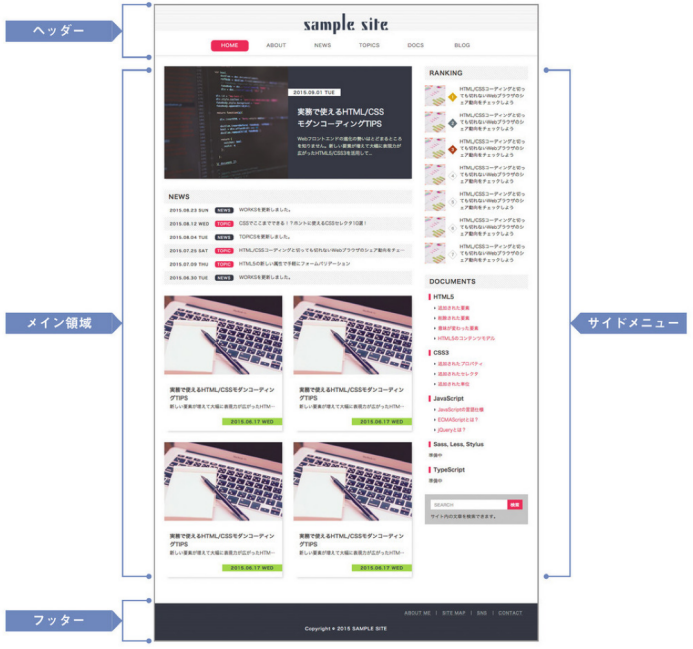
\includegraphics{./PART2/Fig/Fig01_01.PNG}}\vspc{-0.50zw}\caption{このPartで制作するサイトのデザイン}\label{このPartで制作するサイトのデザイン}\end{figure}\vspc{-1.50zw}
%%
%% 節:このレイアウトの特徴
%%--------------------------------------------------------------------------------------------------------------------%%
\section{このレイアウトの特徴}
世の中には様々な形の Web サイトが存在するが、その中でも多くのサイトに当てはまるのが「ヘッダー、フッター、サイドメニュー、メイン領域」を持つレイアウトである。\\

サイト内で共通となるヘッダー、フッター、サイドメニューにサイト内の各コンテンツへのリンクを配置することで全てのページから効率的に各コンテンツへの導線を引くことができるため、ポータルサイト、コーポレートサイト、ショッピングサイト、ニュースサイト、ブログなど情報量が多くページ数の多いサイトに向いている。\\

閲覧者にとっても見慣れたレイアウトなので、どこがメインのコンテンツであるかが直感的に把握でき、視線が迷うことが少ないという特徴がある。\enlargethispage{0.50zw}
その反面、第一印象のインパクトには欠けるため、トップページは個性的なレイアウトで印象的なビジュアルにし、下層ページからこのスタンダードなレイアウトに切り替えるパターンも見られる。
%%
%% 節:サイトを構成する要素
%%--------------------------------------------------------------------------------------------------------------------%%
\section{サイトを構成する要素}
\vspc{-1.50zw}\begin{longtable}[l]{@{}ll@{}}                                                                  \\[-1.30zw]
  \hspc{+2.00zw}\large{\textcolor{blue}{ヘッダー}}                 & \large{\textcolor{blue}{サイドメニュー}} \\
  \hspc{+2.00zw}$\bullet$サイトロゴ                                & $\bullet$ランキング                      \\
  \hspc{+2.00zw}$\bullet$ナビゲーションメニュー                    & $\bullet$ドキュメントリスト              \\
  \hspc{+2.00zw}{~}                                                & $\bullet$検索ボックス                    \\
  \hspc{+2.00zw}\large{\textcolor{blue}{メイン領域}}\hspc{+2.00zw} & {~}                                      \\
  \hspc{+2.00zw}$\bullet$特集コンテンツ                            & \large{\textcolor{blue}{フッター}}       \\
  \hspc{+2.00zw}$\bullet$更新履歴                                  & $\bullet$フッターメニュー                \\
  \hspc{+2.00zw}$\bullet$記事ブロック                              & $\bullet$コピーライト                    \\
\end{longtable}\vspc{-1.50zw}
\vspc{-5.00pt}\begin{figure}[H]\centering\scalebox{0.40}{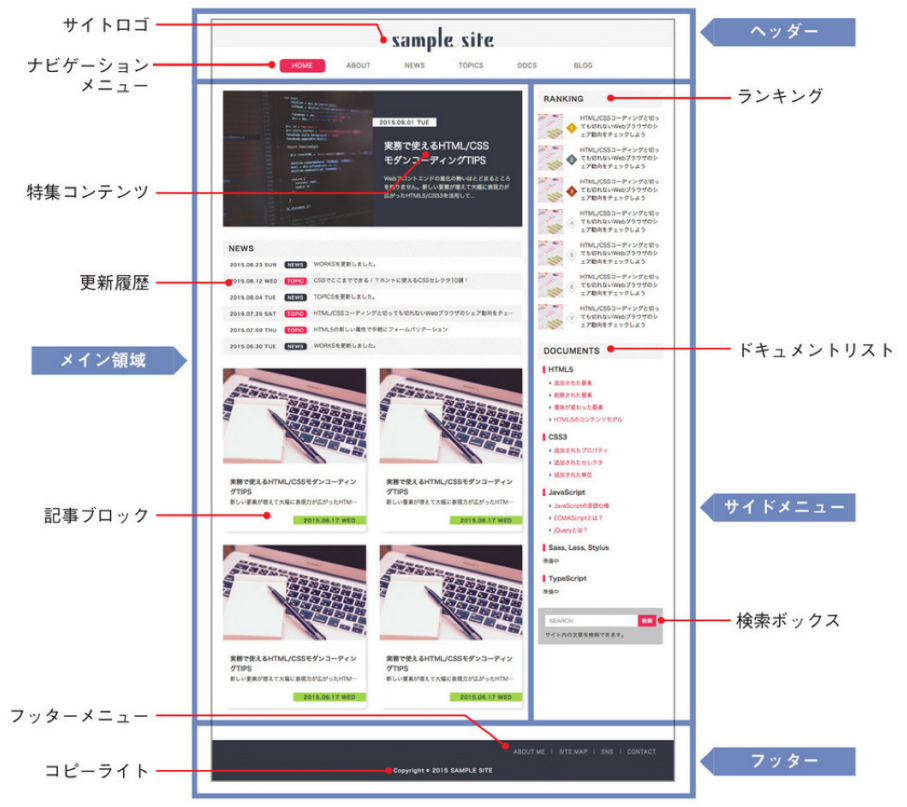
\includegraphics{./PART2/Fig/Fig01_02.PNG}}\end{figure}\vspc{-1.50zw}
本 Part では、このスタンダードなレイアウトで Web フロントエンド技術の情報サイトのトップページを制作する。
